\documentclass[12pt]{iopart}
\pdfminorversion=4
\usepackage{graphicx}
%Uncomment next line if AMS fonts required
%\usepackage{iopams}
\usepackage{myphysics} %units, particles and misc definitions from ATLAS
\usepackage{graphicx}  %\includegraphics...

\begin{document}

\title[Electroweak phyiscs at the LHC]{Electroweak physics at the LHC}
\author{J Berryhill$^1$ and A Oh$^2$}

\address{$^1$ Fermi National Accelerator Laboratory, Batavia, IL, USA}
\address{$^2$ School of Physics and Astronomy, University of Manchester, Manchester, UK}

%\ead{submissions@iop.org}
%\vspace{10pt}
%\begin{indented}
%\item[]February 2014
%\end{indented}

\begin{abstract}
The Large Hadron Collider (LHC) has completed in 2012 its first
running phase and the experiments have collected data sets of pp
collisions at center-of-mass energies of 7 and 8 \TeV\xspace with an
integrated luminosity of about 5 \ifb and 20 \ifb, respectively.  Analyses
of these data sets have produced a rich set of results in the
electroweak sector of the standard model. This article reviews the
status of electroweak measurements of the ATLAS and CMS experiments at
the LHC and discusses phenomenological developments in the electroweak
sector.
\end{abstract}

% Uncomment for PACS numbers
\pacs{12.15.-y, 12.60.Cn, 14.70.-e}
%
% Uncomment for keywords
%\vspace{2pc}
%\noindent{\it Keywords}: XXX, YYY, ZZZ
%
% Uncomment for Submitted to journal title message
\submitto{\jpg}
%
% Uncomment if a separate title page is required
\maketitle
%
% For two-column output uncomment the next line and choose [10pt] rather than [12pt] in the \documentclass declaration
%\ioptwocol
%


\section{Introduction}
\subsection{Motivation to study the electroweak sector}
\subsection{Electroweak physics at hadron colliders}
\subsection{LHC physics program}
\subsection{Electroweak challenges for Run 2 and beyond}

\section{Theory overview and recent developments}
\subsection{PDF and electroweak observables (V+jets, $\phi^*$)}
\subsection{Electroweak NLO corrections}
\subsection{Anomalous gauge couplings and effective field theory}
\subsection{Oblique corrections, constructed observables}


\section{Inclusive boson production}
\subsection{Drell-Yan production}
\label{ss-inclboson-drellyan}
At a hadron collider, the most fundamental tests of electroweak boson
couplings to fermions are measurements of the kinematic properties of
Drell-Yan (DY) lepton pair production.  At leading order, Drell-Yan
production occurs when a quark--anti-quark pair in the initial state
annihilates into an electroweak boson, which subsequently decays to a
lepton pair. Differential cross section calculations exist for
next-to-next-to leading order (NNLO) QCD corrections as well as NLO
electroweak corrections. In the EFT context, such a process is
sensitive to four-fermion contact interactions of the type

\begin{equation}\label{lagrangian}
\begin{array}{r@{\,}c@{}c@{\,}l@{\,}l}
\mathcal L = \frac{g^2}{\Lambda^2}\;[ && \eta_{\rm LL}&\, (\overline q_{\rm L}\gamma_{\mu} q_{\rm L})\,(\overline\ell_{\rm L}\gamma^{\mu}\ell_{\rm L}) \nonumber \\
& +&\eta_{\rm RR}& (\overline q_{\rm R}\gamma_{\mu} q_{\rm R}) \,(\overline\ell_{\rm R}\gamma^{\mu}\ell_{\rm R}) \\
&+&\eta_{\rm LR}& (\overline q_{\rm L}\gamma_{\mu} q_{\rm L}) \,(\overline\ell_{\rm R}\gamma^{\mu}\ell_{\rm R}) \\
&+&\eta_{\rm RL}& (\overline q_{\rm R}\gamma_{\mu} q_{\rm R}) \,(\overline\ell_{\rm L}\gamma^{\mu}\ell_{\rm L})& ] \: ,\nonumber
\end{array}
\end{equation}
where $g$ is a coupling constant, $\Lambda$ is the contact interaction scale,
and $q_{\rm L,R}$ and $\ell_{\rm L,R}$ are left-handed and right-handed quark and
lepton fields, respectively. The parameters $\eta_{i,j}$ denote the relative interference of the operators;
the experiments have considered the cases $\eta_{\rm LR} = \eta_{\rm RL} = \pm 1$,
$\eta_{\rm LL} = \pm 1$, or $\eta_{\rm RR} = \pm 1$.

Experiments select electron or muon pairs above trigger thresholds:
CMS selects leading lepton $\pt >$ 17 GeV and second leading lepton
$\pt >$ 8 GeV inclusively, and ATLAS selects high mass events with
both lepton $\pt >$ 25 GeV.  Backgrounds to Drell-Yan production are
relatively small, and consist of real prompt lepton pair production
from top quark or boson pairs, as well as fake electrons from QCD
jets.  The real lepton pair background is flavor democratic, and can
therefore be reliably estimated from $e\mu$ pair production.  Fake
electron production is typically estimated from background enriched
QCD jet samples, from which the fake electron rate can be measured,
convolved with electron-jet control samples.

Figure~\ref{fig:ss-inclboson-drellyan-atlas7tev} shows the Drell-Yan
cross section at high electron pair mass measured by ATLAS at 7
TeV~\cite{Aad:2013iua}.  The cross section uncertainty is
predominantly systematic below 400 GeV in pair mass and predominantly
statistical above 400 GeV.  The data are compared with an NNLO QCD
prediction with NLO electroweak corrections, provided by the
\texttt{FEWZ} 3.1
generator~\cite{Melnikov:2006kv,Gavin:2010az,Li:2012wna}.  The
prediction also includes photon induced lepton pair production, which
generally increases cross section estimates by a few percent. The
\texttt{FEWZ} prediction generally underestimates the cross section,
however a correlated chi-squared analysis concludes that this is not
statistically significant.

Figure~\ref{fig:ss-inclboson-drellyan-cms8tev} shows the Drell-Yan
cross section for electron or muon pairs measured by CMS at 8
TeV~\cite{CMS:2014jea}.  Agreement with the \texttt{FEWZ} prediction
is observed over the entire measured mass range, from 15 GeV to 2000
GeV.  CMS has also measured the double differential cross section with
respect to dilepton rapidity in several bins of dilepton mass, as well
as a differential cross section ratio between the 8 TeV and 7 TeV
data, which has small experimental and theoretical uncertainties.

In the absence of observed disagreements with predictions at the
highest dilepton masses, the data are analyzed to constrain the size
of anomalous contact interactions. Assuming a fixed, strong value for
the coupling ($g^2/4\pi = 1$), limits can be obtained on the contact
interaction scale $\Lambda$.  ATLAS estimates a lower limit of 17 to
26 TeV on $\Lambda$, where the strongest lower limits correspond to
constructive interference scenarios (especially LR+RL), and the
weakest to destructive interference scenarios~\cite{Aad:2014wca}. CMS
has limits with similar sensitivity estimated for LL contact
interactions~\cite{Khachatryan:2014fba}.

%ATLAS low-mass Drell-Yan $7 \TeV$~\cite{Aad:2014qja}
%ATLAS Z PT $7 \TeV$~\cite{Aad:2014xaa}
%ATLAS Z phistar $7 \TeV$~\cite{Aad:2012wfa}
%CMS Drell--Yan $7 \TeV$~\cite{Chatrchyan:2013tia}
%CMS angular coefficients $8 \TeV$~\cite{Khachatryan:2015paa}
%CMS Z PT and rapidity $8 \TeV$~\cite{Khachatryan:2015oaa}
%CMS dilepton contact interactions~\cite{Khachatryan:2014fba}
%ATLAS dilepton contact interactions~\cite{Aad:2014wca}

\begin{figure}[p]
    \centering
    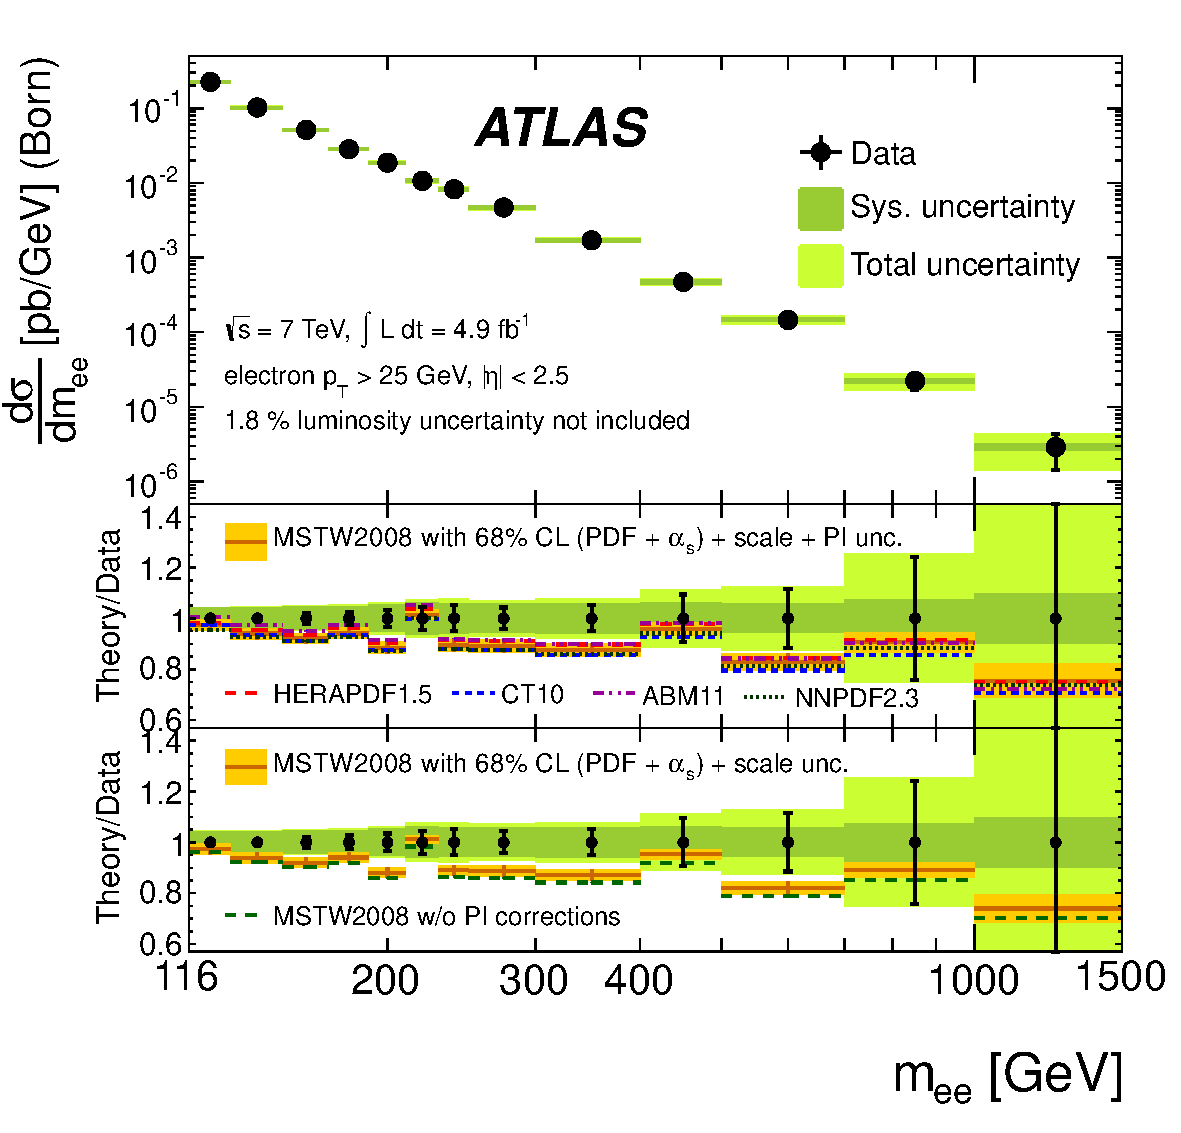
\includegraphics[height=0.3\textheight]{figures/ss-inclboson-drellyan-atlas7tev}
    \caption{Measured differential cross-section at the Born level within the
    fiducial region (electron $\pt > 25 \GeV$ and $|\eta| < 2.5$) with statistical,
     systematic, and combined statistical and systematic (total) uncertainties,
     excluding the 1.8\% uncertainty on the luminosity from ATLAS~\cite{Aad:2013iua}.
     In the upper ratio plot, the photon-induced (PI)
     corrections have been added to the predictions obtained from the MSTW2008,
     HERAPDF1.5, CT10, ABM11 and NNPDF2.3 NNLO PDFs, and for the MSTW2008 prediction
     the total uncertainty band arising from the PDF, $\alpha_s$, renormalisation
     and factorization scale, and photon-induced uncertainties is drawn. The lower
     ratio plot shows the influence of the photon-induced corrections on the
     MSTW2008 prediction, the uncertainty band including only the PDF, $\alpha_s$
     and scale uncertainties.}
    \label{fig:ss-inclboson-drellyan-atlas7tev}
\end{figure}

\begin{figure}[p]
    \centering
    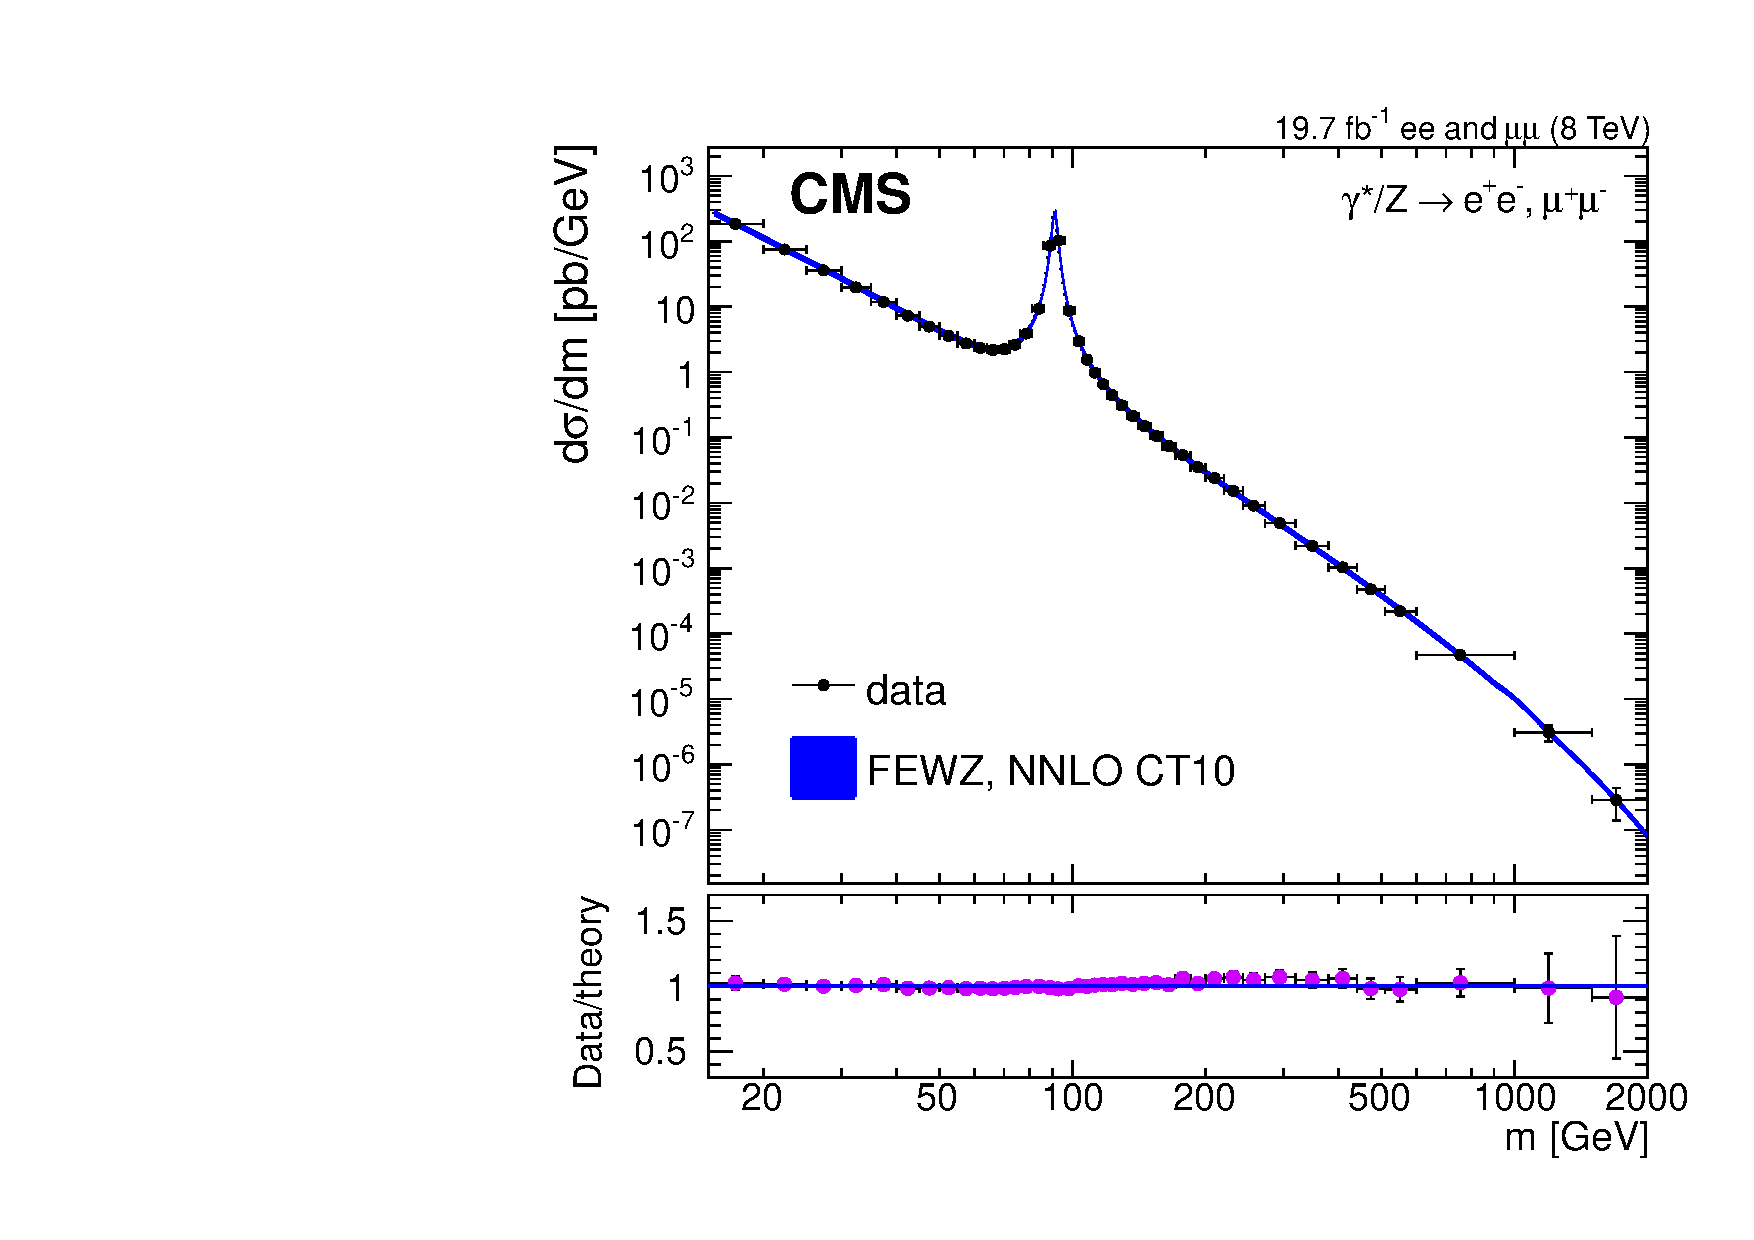
\includegraphics[height=0.3\textheight]{figures/ss-inclboson-drellyan-cms8tev}
    \caption{The DY differential cross section as measured by CMS~\cite{CMS:2014jea} in the combined
dilepton channel and as predicted by NNLO \texttt{FEWZ} 3.1 with CT10 PDF
calculations, for the full phase space.}
    \label{fig:ss-inclboson-drellyan-cms8tev}
\end{figure}

\subsection{Inclusive di-boson production}

ATLAS \Wg \Zg 7 \TeV\xspace~\cite{Aad:2013izg}

CMS \Wg/\Zg 7 \TeV\xspace~\cite{Chatrchyan:2013fya}

CMS $Z(\nu\bar{\nu})\gamma$ 7 \TeV~\cite{Chatrchyan:2013nda}

CMS \Zg 8 \TeV~\cite{Khachatryan:2015kea}


ATLAS simultaneous tt/WW/Z cross section 7 \TeV~\cite{Aad:2014jra}

ATLAS WW 7 \TeV~\cite{ATLAS:2012mec}

ATLAS WW+WZ cross section 7 \TeV~\cite{Aad:2014mda}

ATLAS WW 8 \TeV~\cite{ATLAS-CONF-2014-033}

CMS WW2l2n 7 \TeV~\cite{Chatrchyan:2013yaa}

CMS WWlnjj 7 \TeV~\cite{Chatrchyan:2012bd}

CMS WW/ZZ 8 \TeV~\cite{Chatrchyan:2013oev}

CMS WW2l2n 8 \TeV (CMS-PAS-SMP-14-016, to be published)


ATLAS WZ 7 \TeV~\cite{Aad:2012twa}

CMS VZ 8 \TeV~\cite{Chatrchyan:2014aqa}

CMS WZ at 7+8 \TeV (CMS-PAS-SMP-12-006, to be published)

\subsubsection{ZZ production}
\label{sss-ZZprod}


\subsubsection{ZZ production}
\label{sss-ZZprod}

%short intro
The production of \ZZ in proton-proton collisions has been one of the first di-boson 
processes measured at the LHC. The SM process is and an important and irreducible
background to resonance searches and Higgs production. The production at leading
order is dominated by quark anti-quark annihilation in the $t$ and $u$-channel,
whereas the $s$-channel process is forbidden in the SM 
(see also Figure~\ref{fig:sss-ZZprod-LOdiagrams}). The gluon fusion process 
contributes about 6\% to the total production cross section. 

%FIGURE LO ZZ DIAGRAM
\begin{figure}[htbp]
  \begin{center}
  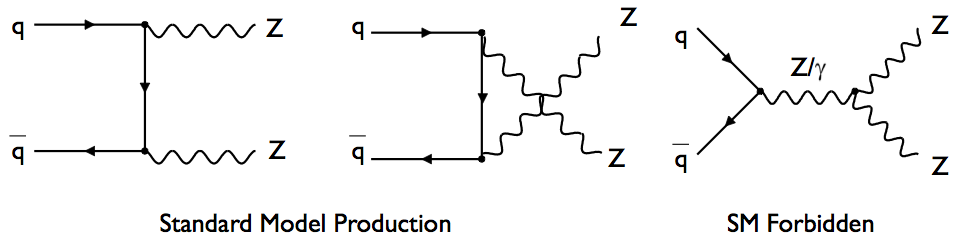
\includegraphics[width=0.9\textwidth]{figures/sss-inclboson-diboson-zzprod-zzdiagram.png}
  \caption{Leading order Feynman diagrams of \ZZ production in the dominant 
  \qqbar\ channel. The \ZZ\ production via the $s$-channel is not allowed in the SM.}
\label{fig:sss-ZZprod-LOdiagrams}
\end{center}
\end{figure}

%decay channels
Precision measurements use the leptonic decay modes of the $Z$ to reduce the impact of
QCD backgrounds. 
The four lepton final state provides an almost background free signature, at the
expense of a relatively small branching ratio 
$BR(ZZ) \to \ll\ll = 0.101^2 \cdot {4 \over 9} = 0.0045$~\cite{PDG}.  
The di-lepton and missing energy channel can exploit the one order of magnitude
higher branching ratio of 
$BR(\ZZ \to \ll\vv) = 0.101 \cdot 0.20 \cdot 2 \cdot {2 \over 3} = 0.0269$, 
at the expense of high background levels.

%analysis CMS and ATLAS.
%ATLAS ZZ 7 TeV~\cite{Aad:2012awa}
%CMS ZZ4l 8 TeV~\cite{Khachatryan:2014dia}
%CMS ZZ4l 7 TeV~\cite{Chatrchyan:2012sga}
%CMS ZZ2l2nu 7+8 TeV~\cite{Khachatryan:2015pba}
The ATLAS collaboration has published results on the $7\TeV$ data-set 
in the $\ll\ll$ and $\ll\vv$ final state~\cite{Aad:2012awa}, and at
$13\TeV$ in the $\ll\ll$ final state~\cite{Aad:2015zqe}. The CMS collaboration
has analysed the full 7 and $8\TeV$ data sets in both 
the $\ll\ll$~\cite{Chatrchyan:2012sga,Khachatryan:2014dia} and 
$\ll\vv$ final state~\cite{Khachatryan:2015pba}.

%Theoretical calculations
% NLO alpha_s arXiv:1105.0020
% NLO alpha_EKW arXiv:1305.5402,arXiv:1307.4331
Theoretical predictions for $\ZZ$ production are available 
at NLO in $\alpha_s$~\cite{arXiv:1105.0020}. In addition, electroweak 
corrections at NLO have been calculated~\cite{arXiv:1305.5402,arXiv:1307.4331}. 

% Z->llll
%Selections
The event selection for the $\ll\ll$ final state requires exactly four leptons 
fulfilling a set of cuts on kinematic quantities. ATLAS and CMS use similar criteria 
as listed in detail in Table~\ref{tab:sss-ZZprod-cuts}. While ATLAS uses $l=e,\mu$,
CMS includes also $\Z\to\tautau$ with subsequent hadronic and leptonic $\tau$
decays. ATLAS uses in addition forward leptons outside the ID tracker
to increase the acceptance by 6\% for electrons and 10\% for muons.
%Backgrounds
The $\ll\ll$ channels offers the cleanest event sample with a background level
of only $2-3\%$ from $\Z+jets$, $\tt$, and di-boson events. 
The background is estimated from data by control regions with looser selection
criteria. 

% Z->llvv
%Selections
Events in the $\ll\vv$ final state are characterized by exactly two leptons 
and missing energy. The event selection requires a leptonic $\Z$ candidate and
missing energy in the event. Both experiments used refined observables of
missing energy with additional information to improve the rejection 
against instrumental background. 
%Backgrounds 
The background level is in the same order
as the signal and substantially higher then for $\ll\ll$ .
Main background sources are $\V+jets$, $\tt$ and di-boson production. 
ATLAS and CMS use data driven techniques to constrain the 
dominant background sources.

% Results at the end?
% xsec
Besides the total cross section for the $pp \to \ZZ$ production process, both
experiments measure also fiducial and differential cross sections. The results are 
summarized in Tabel~\ref{tab:sss-ZZprod-cross-sections}. ATLAS and CMS
use different definitions of the fiducial phase space which needs to be taken into
account to make a direct comparison is possible.
For the total cross section a slightly different mass range for the $\Z$ mass range is
used, where CMS uses a wider range of $60\GeV < \mZ < 120\GeV$ then ATLAS with 
$66\GeV < \mZ < 116\GeV$, which contributes to the difference in the quoted predicted
cross section. Good agreement of experimental and theoretical cross section 
values is observed. 


\begin{table}[htp]
\begin{center}
\resizebox{\textwidth}{!}{
\begin{tabular}{|c|c|c|c|c|c|}
 \hline
 Experiment & decay channel     & \rts & measured $\sigma_{total}$ $[\pb]$                                  & predicted $\sigma_{total}$ $[\pb]$& reference                    \\
 \hline
 ATLAS	     & $\ll\ll$, $\ll\vv$& 7 TeV & {6.7 $\pm$ 0.7 (stat.) $^{+0.4}_{-0.3}$ (syst.) $\pm$ 0.3 (lumi.) }&  6.18$^{+0.25}_{-0.18}$           & \cite{Aad:2012awa}         \\
 CMS	     & $\ll\ll$          & 7 TeV & {6.2 $\pm$ $^{+0.9}_{-0.8}$ (stat.) $^{+0.4}_{-0.3}$ (syst.) $\pm$ 0.1 (lumi.) } & 6.3$\pm 0.4$        & \cite{Chatrchyan:2012sga}  \\
 CMS	     & $\ll\vv$          & 7 TeV & {5.2 $\pm$ $^{+1.5}_{-1.4}$ (stat.) $^{+1.4}_{-1.1}$ (syst.) $\pm$ 0.2 (lumi.) } & 6.1$\pm 0.3$        & \cite{Chatrchyan:2012sga}  \\
 CMS	     & $\ll\ll$          & 8 TeV & {7.7 $\pm$ 0.5 (stat.) $^{+0.5}_{-0.4}$ (syst.) $\pm$ 0.2 (lumi.) } 		        & 7.7$\pm 0.6$        & \cite{CMS:2014xja}         \\ 
 CMS	     & $\ll\vv$          & 8 TeV & {6.9 $\pm$ 0.8 (stat.) $^{+1.8}_{-1.4}$ (syst.) $\pm$ 0.3 (lumi.) }			    & 7.6$\pm 0.3$        & \cite{Chatrchyan:2012sga}  \\% m(ll) > 40GeV, m(vv) > 12GeV
 ATLAS	     & $\ll\ll$			 &13 TeV & {16.7 $\pm$ $^{+2.2}_{-2.0}$ (stat.) $^{+0.9}_{-0.7}$ (syst.) $\pm$ $^{+1.o}_{-0.7}$ (lumi.) }&  15.6$^{+0.4}_{-0.4}$           & \cite{Aad:2015zge}         \\

\hline

\end{tabular}
}
\caption{Summary of measured $\ZZ$ production cross sections from ATLAS and CMS
at 7, 8 and 13 TeV centre-of-mass energies in the four lepton and $\ll\vv$ final state.}
\label{tab:sss-ZZprod-cross-sections}
\end{center}
\label{default}
\end{table}%


%%%%
% THIS MIGHT GO INTO THE SECTION ON TGC
% aTGC
% Spectra ATGC
% charged pT : llvv CMS
% m(llll) : llll CMS
% pT(Z) : llll,llvv ATLAS
Limits on ATGC parameters are determined with differential distributions of the 
invariant di-boson mass (CMS, four lepton channel), 
the transverse momentum of the leading lepton (CMS, $\ll\vv$-channel), or
the transverse momentum of the leading \Z (ATLAS, all channels).
A comparison of the measured and predicted differential cross sections in the 
four-lepton invariant mass is shown from CMS in Figure \ref{fig:sss-inclboson-diboson-zzprod-zzinvmass}.
Also shown is the prediction in the presence of a non-zero value of the anomalous coupling
parameter $f_4^Z=0.015$, which shows an enhancement over the SM value at high 
invariant masses. 

%FIGURE ZZ invariant mass
%1406.0113v2.pdf, FIGURE 5
% https://twiki.cern.ch/twiki/pub/CMSPublic/PhysicsResultsSMP13005/fig5tgcA.pdf
% CMS ZZ 4l 8 TeV
\begin{figure}[htbp]
  \begin{center}
  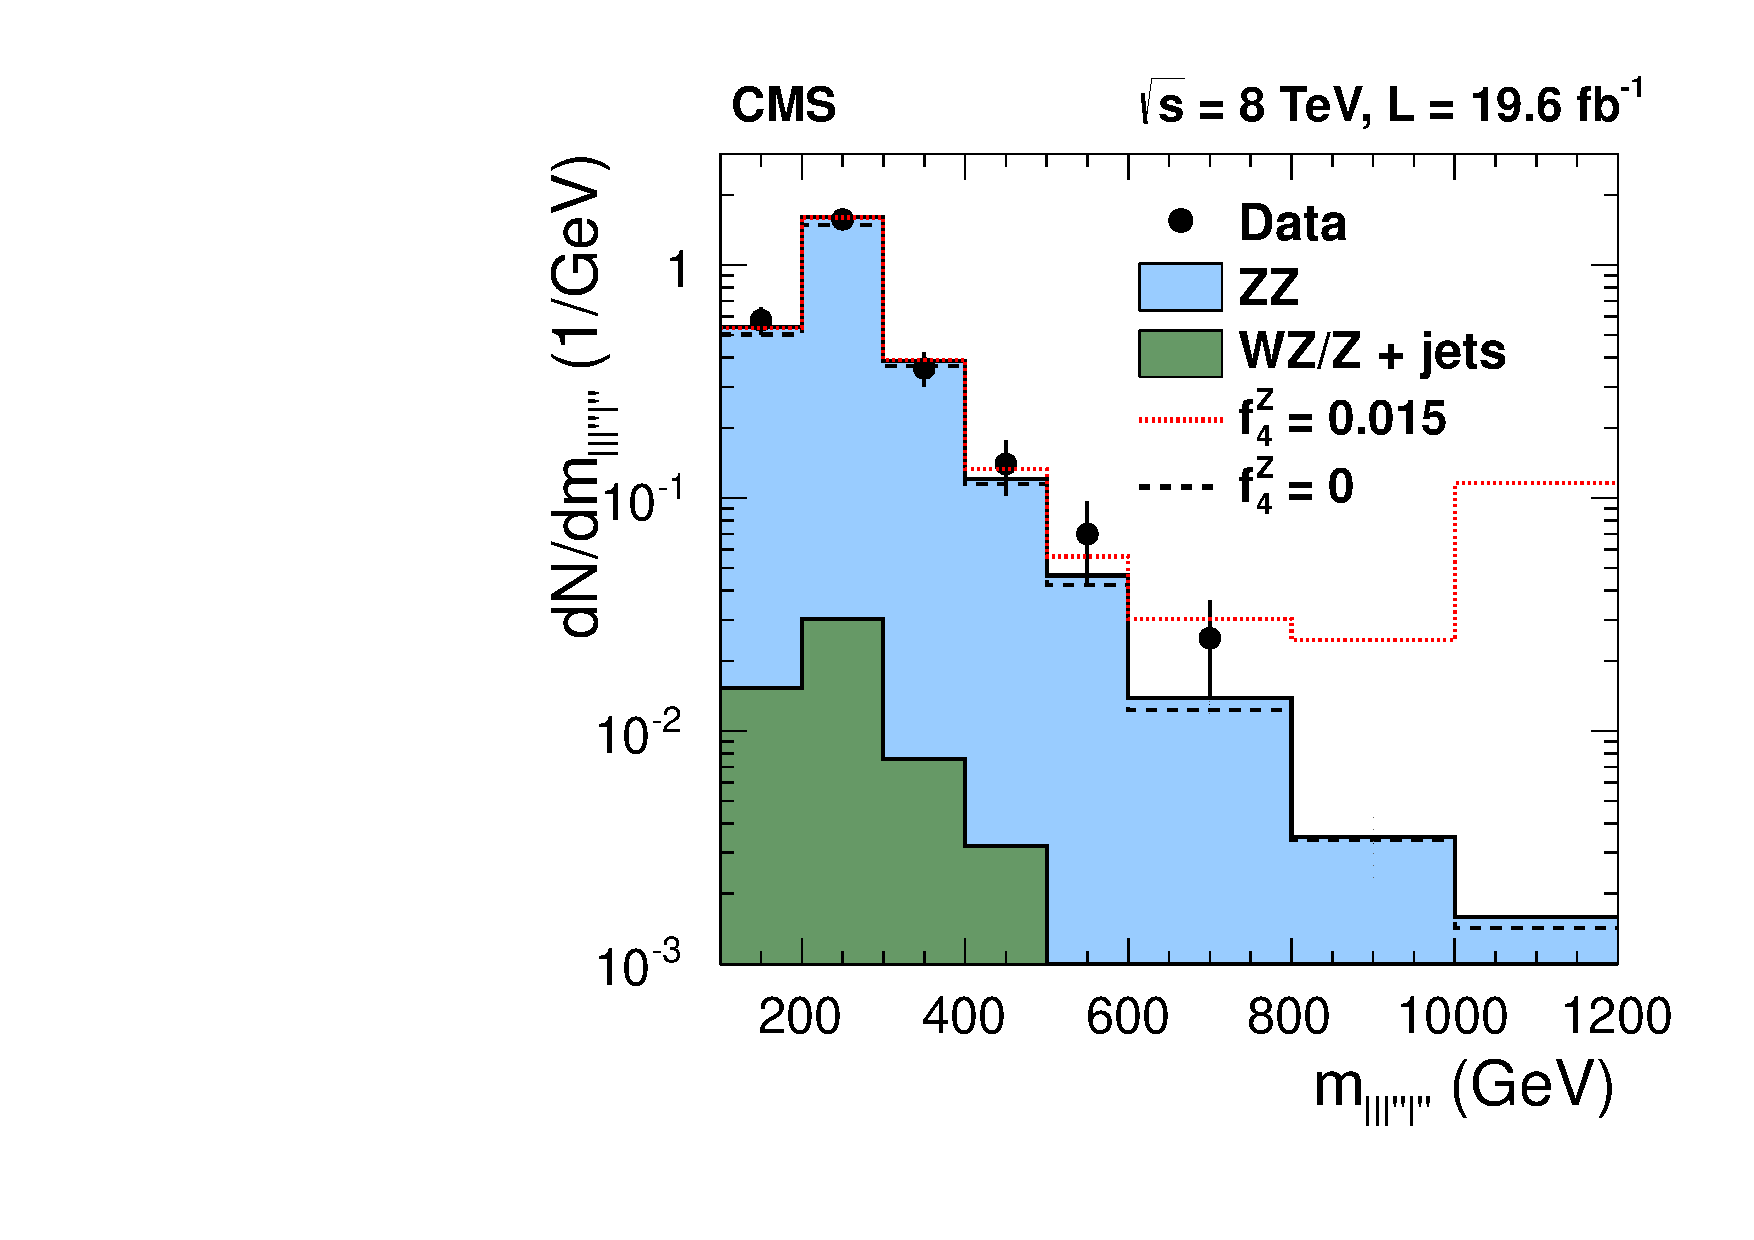
\includegraphics[width=0.9\textwidth]{figures/sss-inclboson-diboson-zzprod-zzinvmass.pdf}
  \caption{ Distribution of the four-lepton reconstructed mass for the combined $4e$, $4\mu$, and $2e2\mu$ channels from CMS~\cite{Khachatryan:2014dia}. Points represent the data, the shaded histogram labeled $\ZZ$ represents the predictions for $\ZZ$ signal, the histograms labeled $\WZ$/$\Z$+jets shows background estimated form data. The dashed and dotted histograms indicate the SM expectation (f4Z = 0) and in the presence of an ATGC (f4Z = 0.015) with all the other anomalous couplings set to zero. The last bin includes all entries with masses above 1000 GeV.
}
\label{fig:sss-inclboson-diboson-zzprod-zzinvmass}
\end{center}
\end{figure}

Both experiment publish 95\% CL limits on ATGC without form factors in the $\ll\ll$ 
and $\ll\vv$ channels. The results are in agreement with the SM and 
summarized in Figure~\ref{fig:sss-inclboson-diboson-zzprod-aTGC_naTGCf} 
taken from Ref. \cite{aTGCplots}. The precision of the LHC results is driven by the steep increase of 
sensitivity with higher centre-of-mass energy
and are about 2 orders of magnitude better compared to the 
combined LEP result~\cite{LEP-comb-2002}.  
% FIGURE COMPARISON OF ZZ NTGC
% https://twiki.cern.ch/twiki/bin/view/CMSPublic/PhysicsResultsSMPaTGC
% M Herndon
% FETCHED 34RD JULY 2015
\begin{figure}[htbp]
  \begin{center}
  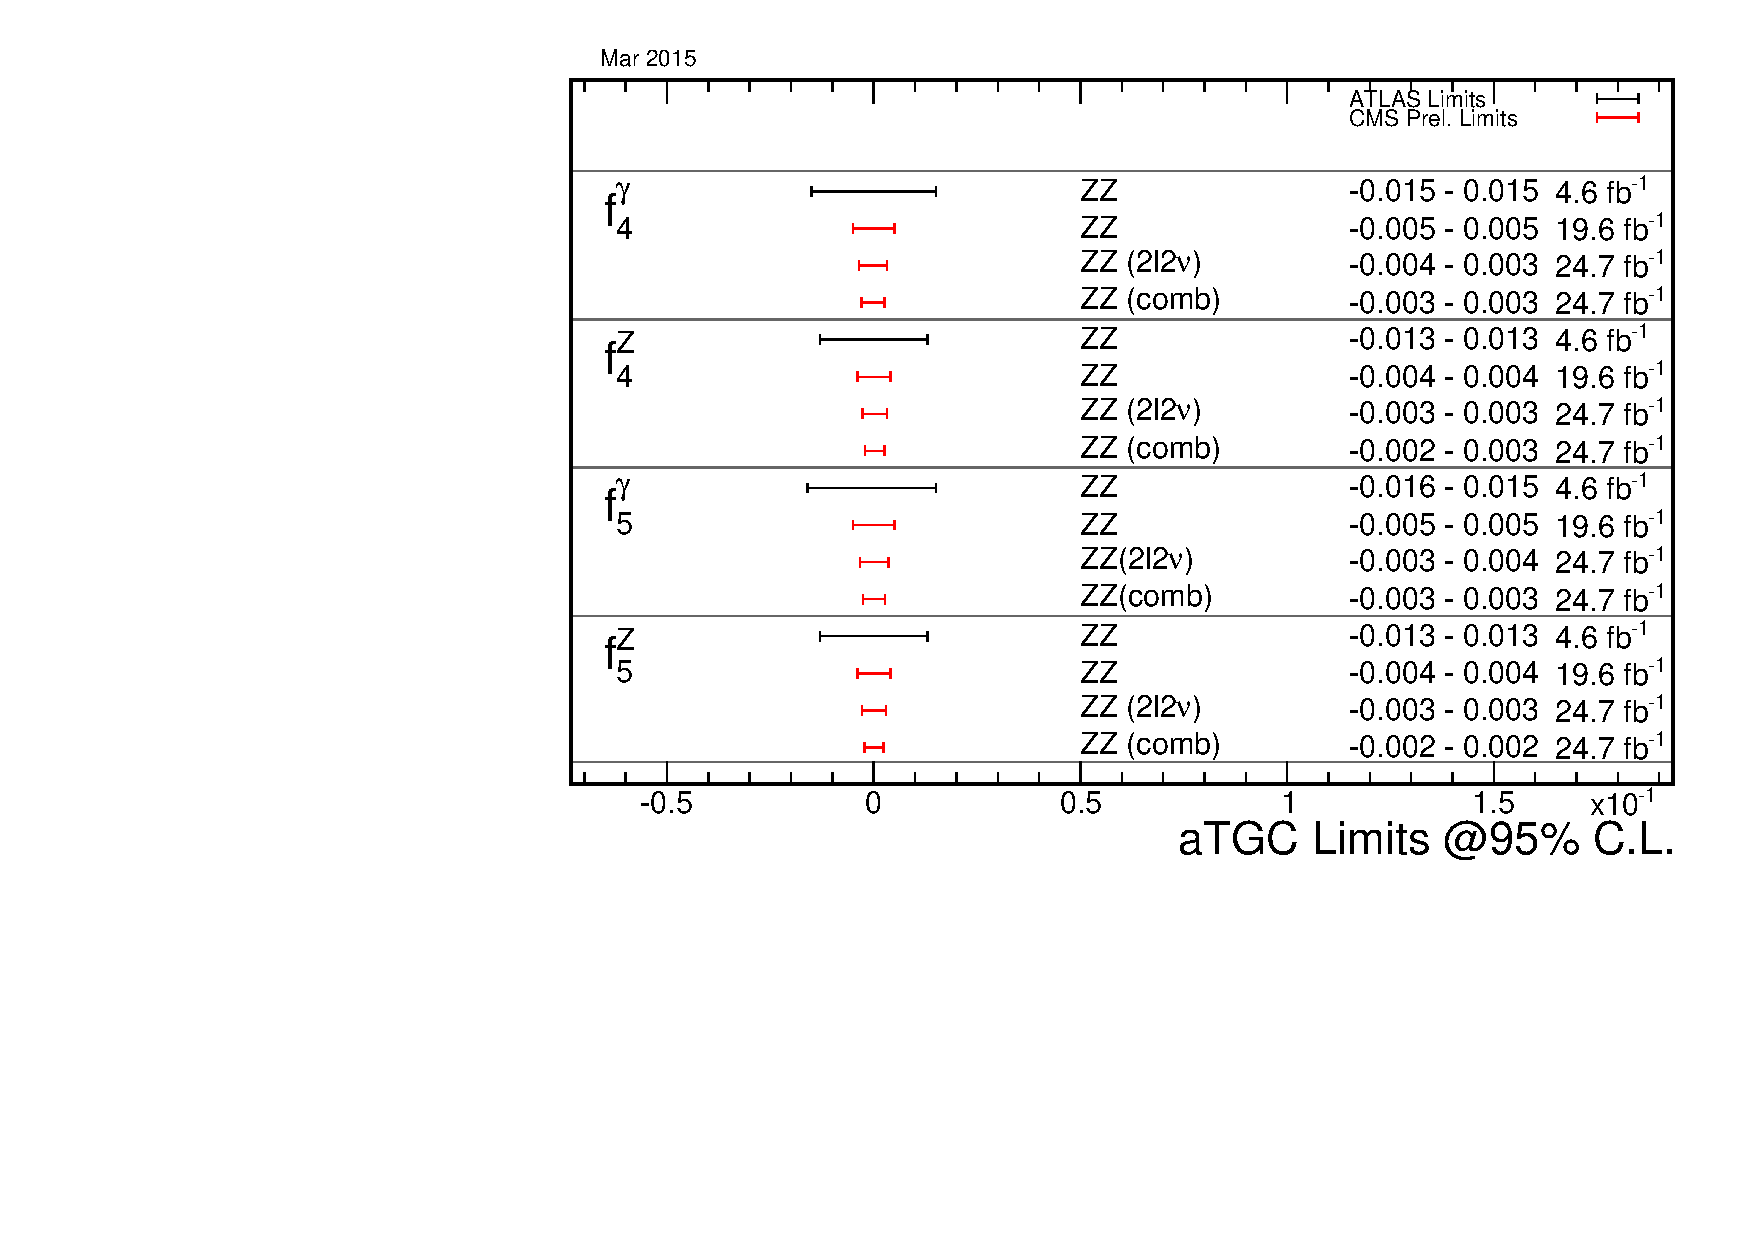
\includegraphics[width=0.9\textwidth]{figures/sss-inclboson-diboson-zzprod-aTGC_naTGCf.pdf}
  \caption{ Comparison of the limits on \ffourv{} and \ffivev{} from ATLAS and CMS in the $\ll\ll$ and $\ll\vv$
  channel at 7 and $8\TeV$.}
\label{fig:sss-inclboson-diboson-zzprod-aTGC_naTGCf}
\end{center}
\end{figure}









%ATLAS ZZ 7 TeV~\cite{Aad:2012awa}
%CMS ZZ4l 8 TeV~\cite{Khachatryan:2014dia}
%CMS ZZ4l 7 TeV~\cite{Chatrchyan:2012sga}
%CMS ZZ2l2nu 7+8 TeV~\cite{Khachatryan:2015pba}




\subsection{Inclusive tri-boson production}

ATLAS $W\gamma\gamma$~\cite{Aad:2015uqa}

CMS WVgamma 8 \TeV~\cite{Chatrchyan:2014bza}

\section{Exclusive boson production}
\subsection{Exclusive single boson production, vector-boson fusion}
\begin{figure}[p]
    \centering
    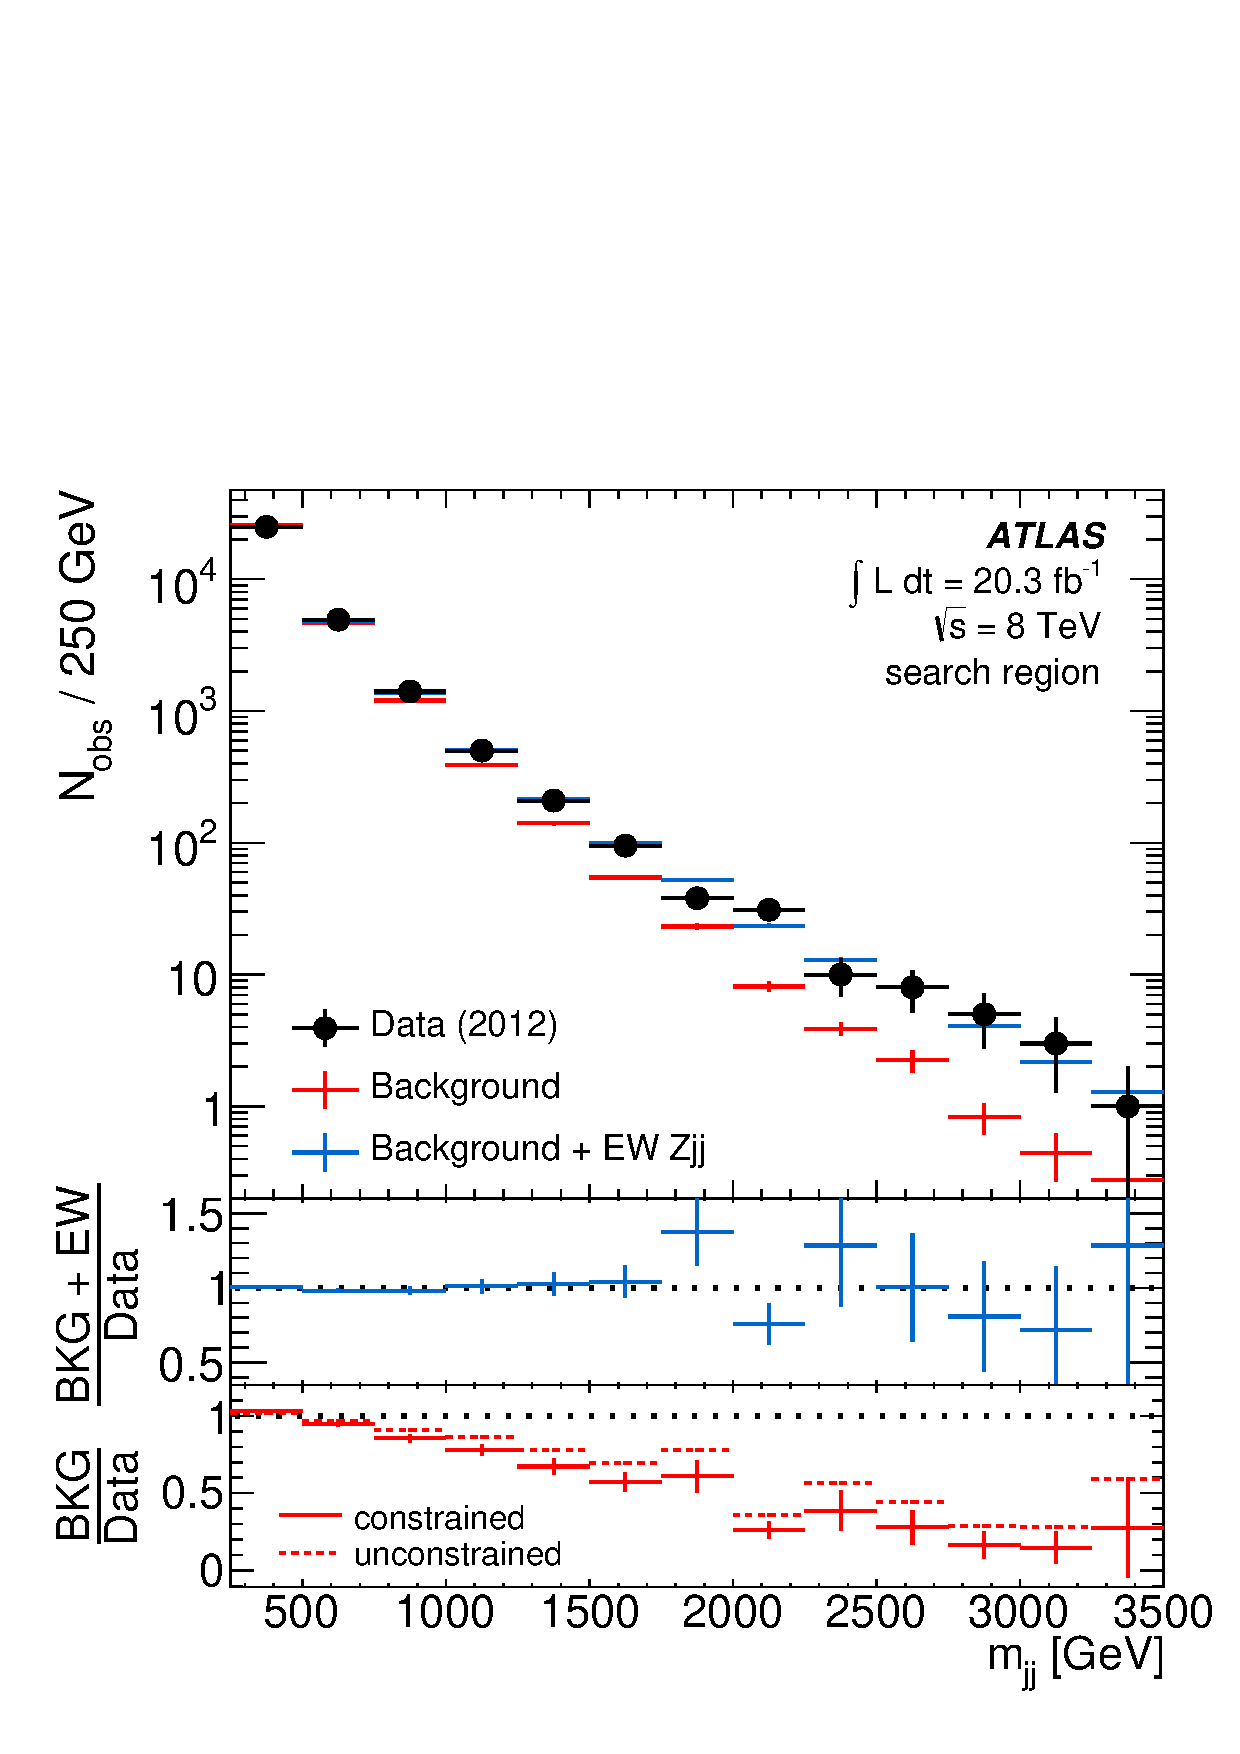
\includegraphics[height=0.3\textheight]{figures/ss-exclboson-z2j-atlas8tev}
    \caption{}
    \label{fig:ss-exclboson-z2j-atlas8tev}
\end{figure}
ATLAS VBF Z 7 \TeV~\cite{Aad:2014dta}

CMS VBF Z 7 \TeV~\cite{Chatrchyan:2013jya}

CMS VBF Z 8 \TeV~\cite{Khachatryan:2014dea}


\subsection{Exclusive di-boson production, vector-boson scattering}
%\begin{figure}[p]
%    \centering
%    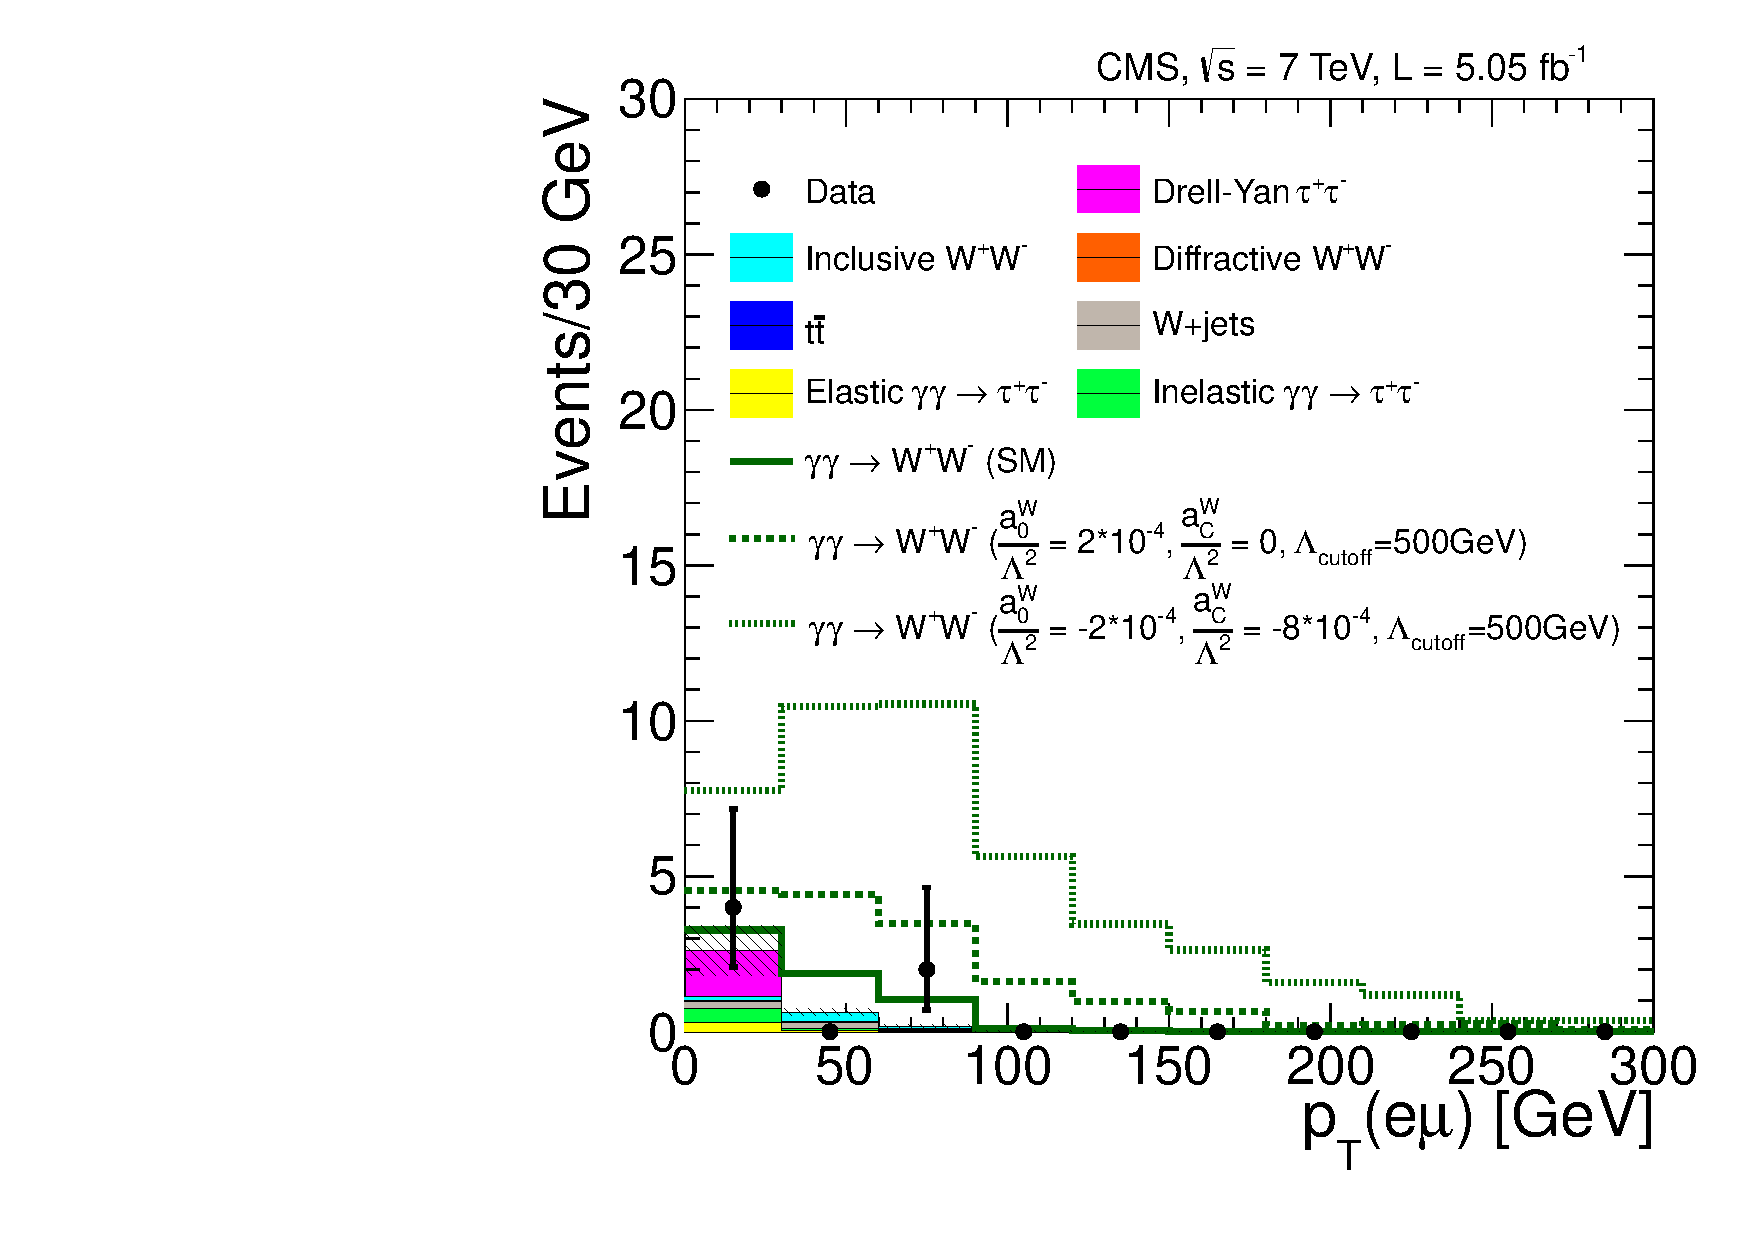
\includegraphics[height=0.3\textheight]{figures/ss-exclboson-ww-cms7tev}
%    \caption{}
%    \label{fig:ss-exclboson-ww-cms7tev}
%\end{figure}
%CMS WWexcl 7 \TeV~\cite{Chatrchyan:2013foa}

In addition to exclusive single boson production, CMS and ATLAS have
evidence for exclusive diboson production, in two different channels.
In one of them, CMS~\cite{Khachatryan:2016mud} has performed a search
for exclusive diboson production via protons emitting (possibly
quasi-) real photons which rescatter to produce $W^+W^-$ pairs:
$pp \to p^{(*)}W^+ W^- p^{(*)} \to p^{(*)}\mu^{\pm}e^{\mp}p^{(*)}$,
where $p^*$ admits the possibility that the protons dissociate into an
undetected system.  Such production is characterized by a
$\mu^{\pm}e^{\mp}$ pair which has no underlying event activity typical
of proton-proton hard scattering.  By selecting a $\mu^{\pm}e^{\mp}$
pair of sufficiently high individual (20 GeV) and joint (30 GeV)
transverse momentum, and requiring further that the two lepton tracks
intersect with each other, but have no additional tracks nearby, an
exclusive production signal is isolated from backgrounds such as
exclusive Drell-Yan and inclusive dilepton production from various
hard scattering mechanisms, respectively.  Selection efficiency is
validated by examining a control sample of exclusive same-flavor
Drell-Yan production ($p^{(*)}\mu^{\pm}\mu^{\mp}p^{(*)}$ or
$p^{(*)}e^{\pm}e^{\mp}p^{(*)}$) and comparing it with simulated
efficiency.  The relative contribution of dissociated proton
scattering for signal is also deduced by comparing the observed
exclusive Drell-Yan cross section with an exclusive matrix element
calculation (\texttt{LPAIR}~\cite{Vermaseren:1982cz,Baranov:1991yq});
proton dissociation is estimated to enhance the signal by a factor of
$4.10 \pm 0.43$ with respect to an exclusive calculation
from \texttt{MadGraph}.

Figure~\ref{fig:ss-exclboson-ww-cms8tev} shows the distributions of
dilepton $\pt$ and extra tracks in data compared with expectations
from simulation.  13 events are observed with an expected background
of $3.9\pm0.6$ in the 8 TeV data.  In the 7
TeV~\cite{Chatrchyan:2013foa} and 8 TeV data combined, a 3.4 $\sigma$
excess is observed over background as evidence for exclusive (plus
dissociative) $W^+W^-$ production.  The signal corresponds to a cross
section in the 8 TeV data of $11.9^{+5.6}_{-4.5}$ fb, in agreement
with a SM prediction of $6.9\pm0.6$ fb.  Exclusive $W^+W^-$ production
is sensitive to $WW\gamma\gamma$ quartic couplings. The CMS analysis
derived limits on the dimension 6 couplings $a^W_0/\Lambda^2$ and
$a^W_C/\Lambda^2$ and, in the context of dimension 8 EFT, the
anomalous couplings $f_{M(0,1,2,3)}/\Lambda^4$.  The 95\% CL upper
limits are $1.1(4.4)\times 10^{-4} \rm{GeV}^{-2}$ for
$a^W_0/\Lambda^2$ ($a^W_C/\Lambda^2$), and range from $2-17 \times
10^{-4} \rm{GeV}^{-4}$ for dimension 8 couplings, for models with no
form factor.  This process is the single best constraint on
$WW\gamma\gamma$ QGCs.

\begin{figure}[htb]
\centering
%\includegraphics[width=.48\textwidth]{Figures/2016_01_29_UpdatedPlots/ee_pt.pdf}
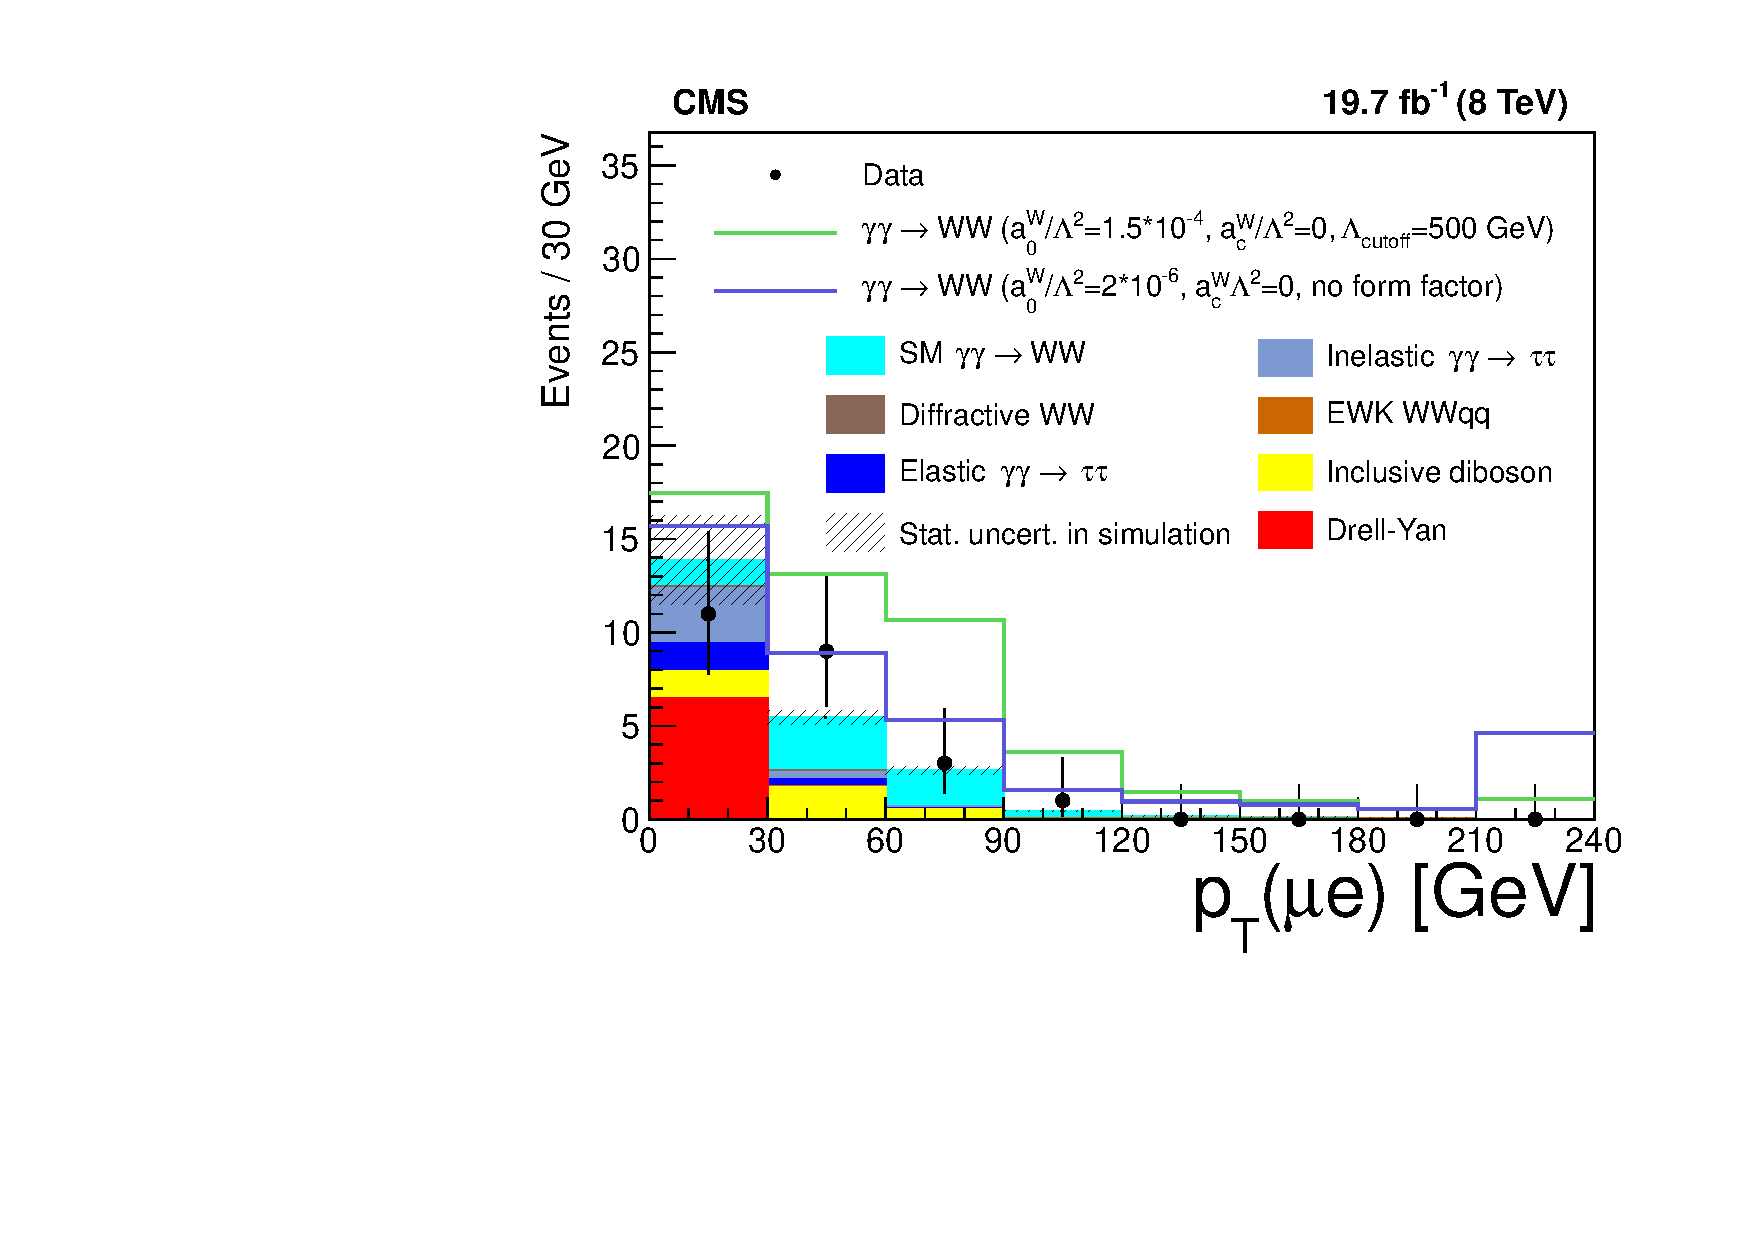
\includegraphics[width=.48\textwidth]{figures/ss-exclboson-ww-cms8tev-1.pdf}
%\includegraphics[width=.48\textwidth]{Figures/2016_01_29_UpdatedPlots/ee_tracks_
%pt30.pdf}
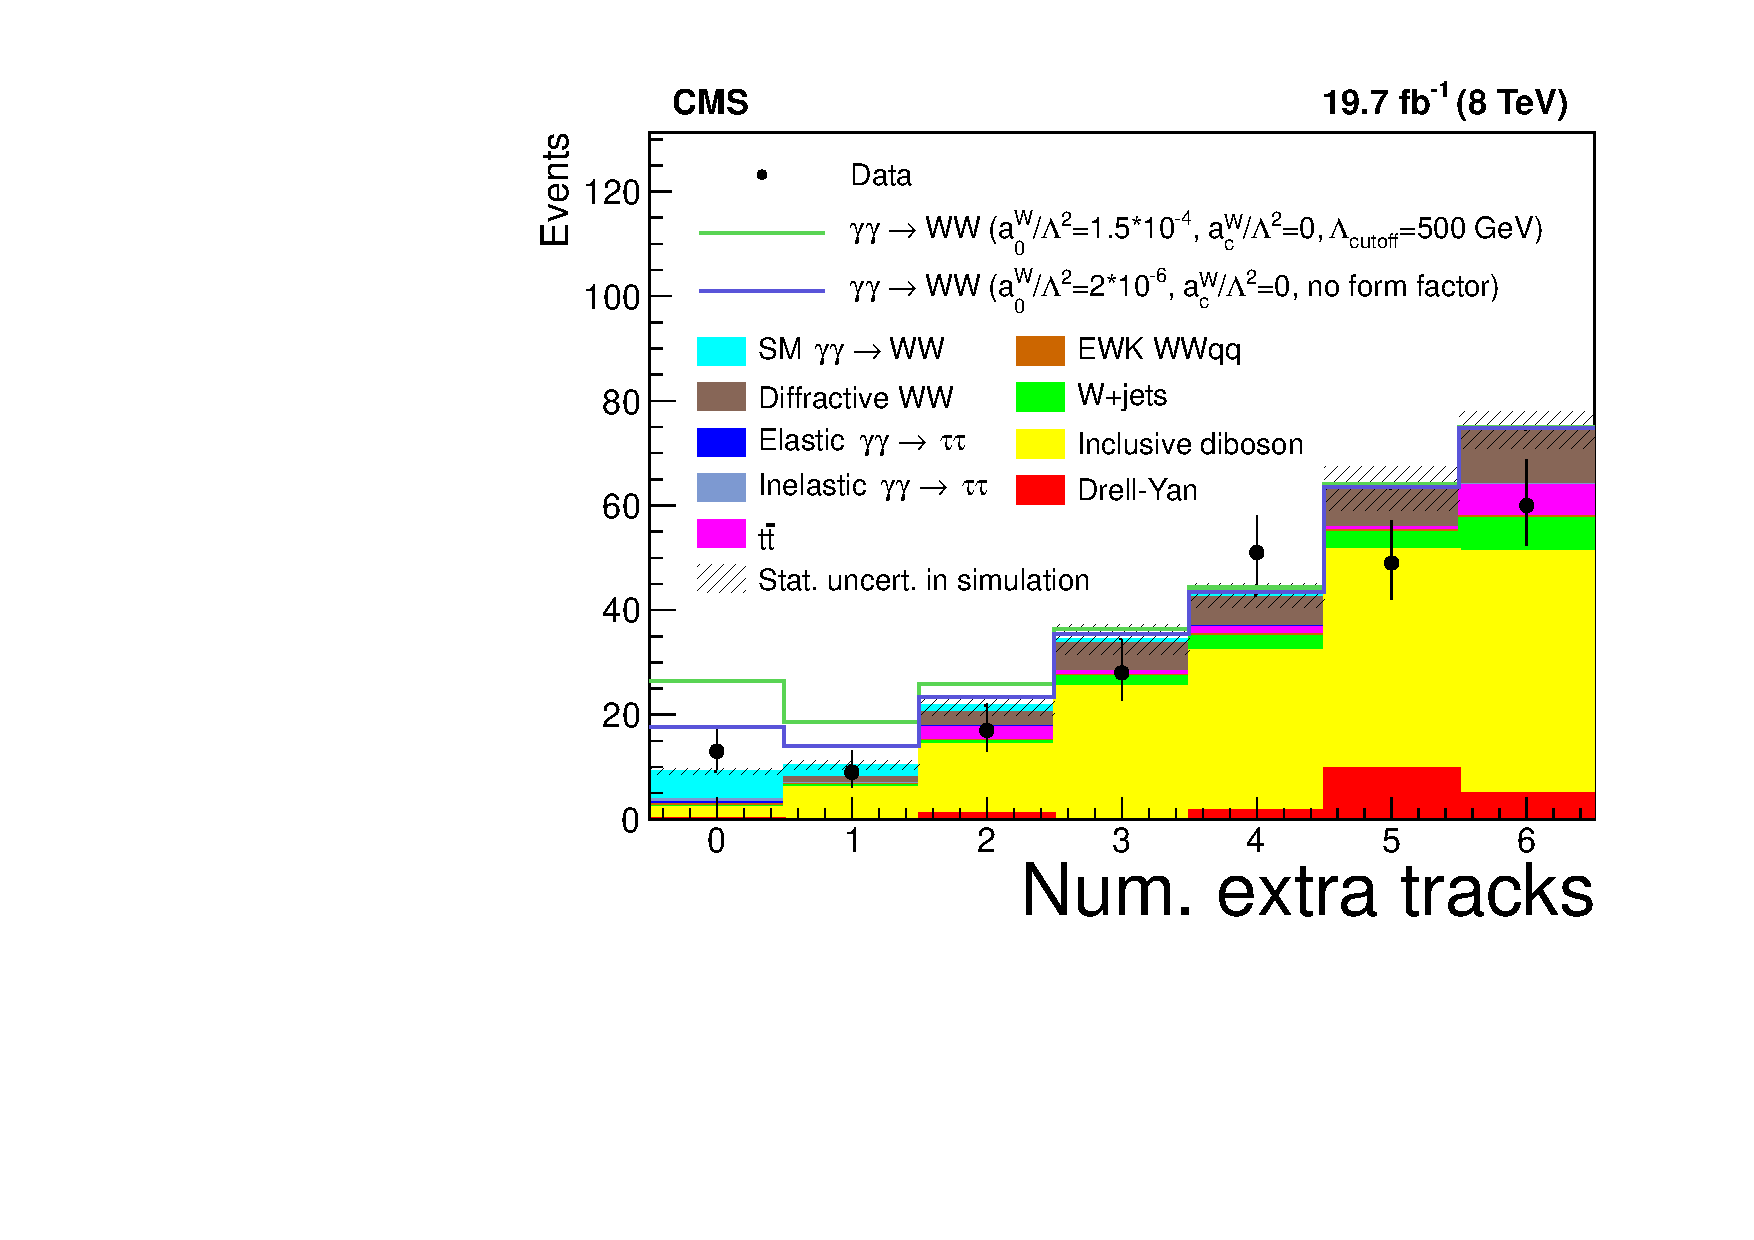
\includegraphics[width=.48\textwidth]{figures/ss-exclboson-ww-cms8tev-2.pdf}
\caption{Evidence for exclusive diboson production via $pp \to p^{(*)}W^+ W^- p^{(*)} \to p^{(*)}\mu^{\pm}e^{\mp}p^{(*)}$~\cite{Khachatryan:2016mud}.
Distributions of muon-electron transverse momentum for events with zero
 associated tracks (left), and extra-tracks multiplicity for events with $\pt(\mu^{\pm}e^{\mp}) > 30$ GeV (right).
 The data are shown by the points with error bars; the histograms indicate the expected SM signal and backgrounds.
\label{fig:ss-exclboson-ww-cms8tev}}
\end{figure}

The other exclusive diboson process for which the LHC has evidence is
same-sign $WW$ production, via the process $qq \to WW +
2q \to \ell^\pm\ell^\pm + 2 \rm{jet} + \met$.  Similar to exclusive
single boson production, the final state of interest is a
superposition of several amplitudes at leading order, some of which
are purely electroweak and include triple and quartic gauge boson
interactions (see Fig.~\ref{fig:ss-exclboson-ww-sigdiagram}), and
some of which have the final state jets arise from QCD initial- and
final-state radiation. Through a suitable choice of final state phase
space, the electroweak amplitudes are enhanced and the associated
signal strength and distributions can be tested against the
electroweak theory.  The same-sign $WW$ final state has the advantage
over other exclusive diboson channels ($\WW$ or $\WZ$) of a smaller
relative QCD amplitude and smaller multi-lepton backgrounds from top
quark, Drell-Yan, and $\WZ$ processes due to the same-sign dilepton
requirement.

An ATLAS analysis~\cite{Aad:2014zda} selects an ``inclusive region''
which is an admixture of electroweak and QCD contributions, and a VBS
signal region which is predominantly electroweak.  The inclusive
region requires two same-sign leptons with $\pt > 25$ GeV, $\met > 40$
GeV, and at least two jets with $m_{jj} > 500$ GeV for the two highest
$\pt$ jets; the VBS region further requires that the two highest $\pt$
jets are separated in rapidity, $|\Delta y_{jj}| > 2.4$.  To reduce
Drell-Yan background, events with dilepton mass less than 20 GeV or
dielectrons within 10 GeV of the $\Zzero$ mass are vetoed.  Top quark
background is reduced by vetoing events with b-tagged jets. Finally,
$WZ$ background is reduced by vetoing events with a third lepton with
muon $\pt > 6$ GeV or electron $\pt > 7$ GeV.  This results in 50
events selected for the inclusive region (as shown in
Fig.~\ref{fig:ss-exclboson-ww-ss}) and 34 for the VBS region.  About
half of selected events in either region are backgrounds from $\WZ$,
$W\gamma$ with photon conversion, and misidentified leptons from jets
in $V$ + jet processes.  The significance of the signal in the
inclusive region is observed (expected) to be 4.5$\sigma$
(3.4$\sigma$), and for the VBS region the significance is observed
(expected) to be 3.6$\sigma$ (2.8$\sigma$).  The measured cross
sections in these two regions are $2.1\pm 0.5\rm{(stat)} \pm
0.3\rm{(syst)}$ fb and $1.3 \pm 0.4\rm{(stat)}\pm 0.2\rm{(syst)}$ fb,
comparing well with SM predictions
from \texttt{Powheg-Box}~\cite{Nason:2004rx,Frixione:2007vw,Alioli:2010xd,Jager:2009xx,Melia:2010bm,Melia:2011gk}
of $1.52 \pm 0.11$ fb and $0.95\pm 0.06$ fb, respectively.

The VBS cross section is used to constrain parameters of an effective
chiral Lagrangian theory of vector boson
scattering~\cite{Alboteanu:2008my}, calculated
by \texttt{Whizard}~\cite{Kilian:2007gr,Moretti:2001zz}: $−0.14
< \alpha_4 < 0.16$ and $−0.23 < \alpha_5 < 0.24$ limits are obtained
at 95\% CL.

A CMS analysis~\cite{Khachatryan:2014sta} selects events similar to
the ATLAS VBS region: two same-sign leptons with $\pt>20$ GeV, two
jets with $m_{jj}>500$ GeV and $|\Delta \eta_{jj}| > 2.5$, and $\met >
40$ GeV.  There is a same-flavor Drell-Yan veto for events with
dilepton mass less than 50 GeV or dielectrons within 15 GeV of the Z
mass, a veto of top-like events with secondary vertex or soft muon
tags, and a third lepton veto for $\pt > 10$ GeV.  The 12 events so
selected are shown in Fig.~\ref{fig:ss-exclboson-ww-ss}.  About half
of them are expected to be background, mostly from misidentified
leptons. The resulting excess has a significance of 1.9$\sigma$
(2.9$\sigma$) observed (expected) for the purely electroweak
amplitude.  The observed fiducial cross section is
$4.0^{+2.4}_{−2.0} \rm{(stat)} ^{+1.1}_{−1.0} \rm{(syst)}$ fb compared
to an expected cross section estimated from \texttt{VBFNLO}~\cite{Baglio:2014uba,Arnold:2011wj,Arnold:2008rz} of
$5.8 \pm 1.2$ fb.

The $m_{\ell\ell}$ distribution of selected events is used to obtain
95\% CL bounds on dimension 8 EFT couplings $f_{S,(0,1)}$,
$f_{M,(0,1,6,7)}$, and $f_{T,(0,1,2)}$~\cite{Eboli:2006wa}.  For
$f_{S,(0,1)}$, which can correspond to a spin-one VBS resonance, the
limits are $-42 \rm{TeV}^{-4} < f_{S,0}/\Lambda^4 < 43 \rm{TeV}^{-4}$
and $-129 \rm{TeV}^{-4} < f_{S,1}/\Lambda^4 < 131 \rm{TeV}^{-4}$.

\begin{figure*}[htb] {
\centering
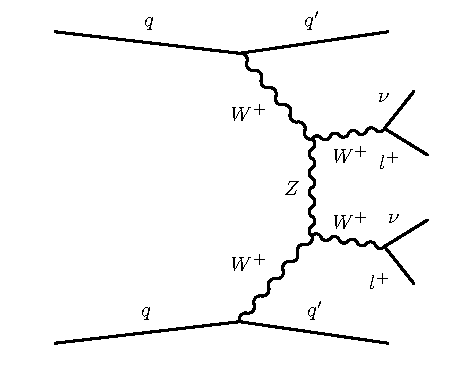
\includegraphics[width=0.315\textwidth]{figures/ss-exclboson-ww-diagram1.pdf}
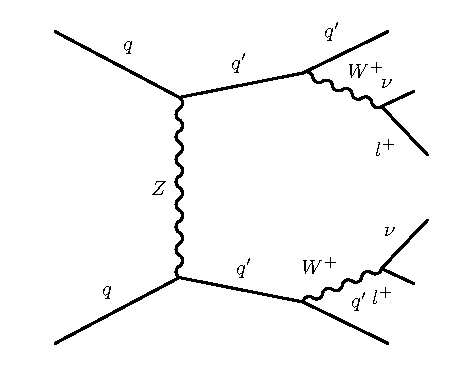
\includegraphics[width=0.35\textwidth]{figures/ss-exclboson-ww-diagram2.pdf}
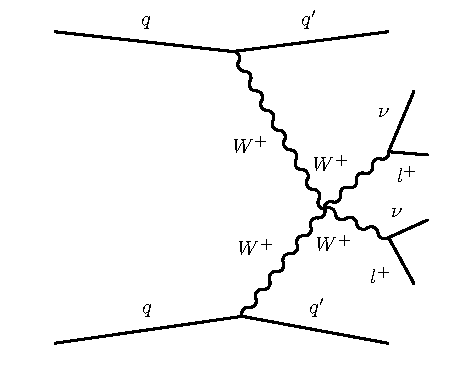
\includegraphics[width=0.315\textwidth]{figures/ss-exclboson-ww-diagram3.pdf}
\caption{
Representative Feynman diagrams for same-sign $WW$ production in association
with two jets from purely electroweak contributions:
(left) vector boson fusion,
(middle) bremsstrahlung-like,
and (right) multiperipheral production~\cite{Khachatryan:2014sta}.
\label{fig:ss-exclboson-ww-sigdiagram}}

}
\end{figure*}


\begin{figure}[p]
    \centering
    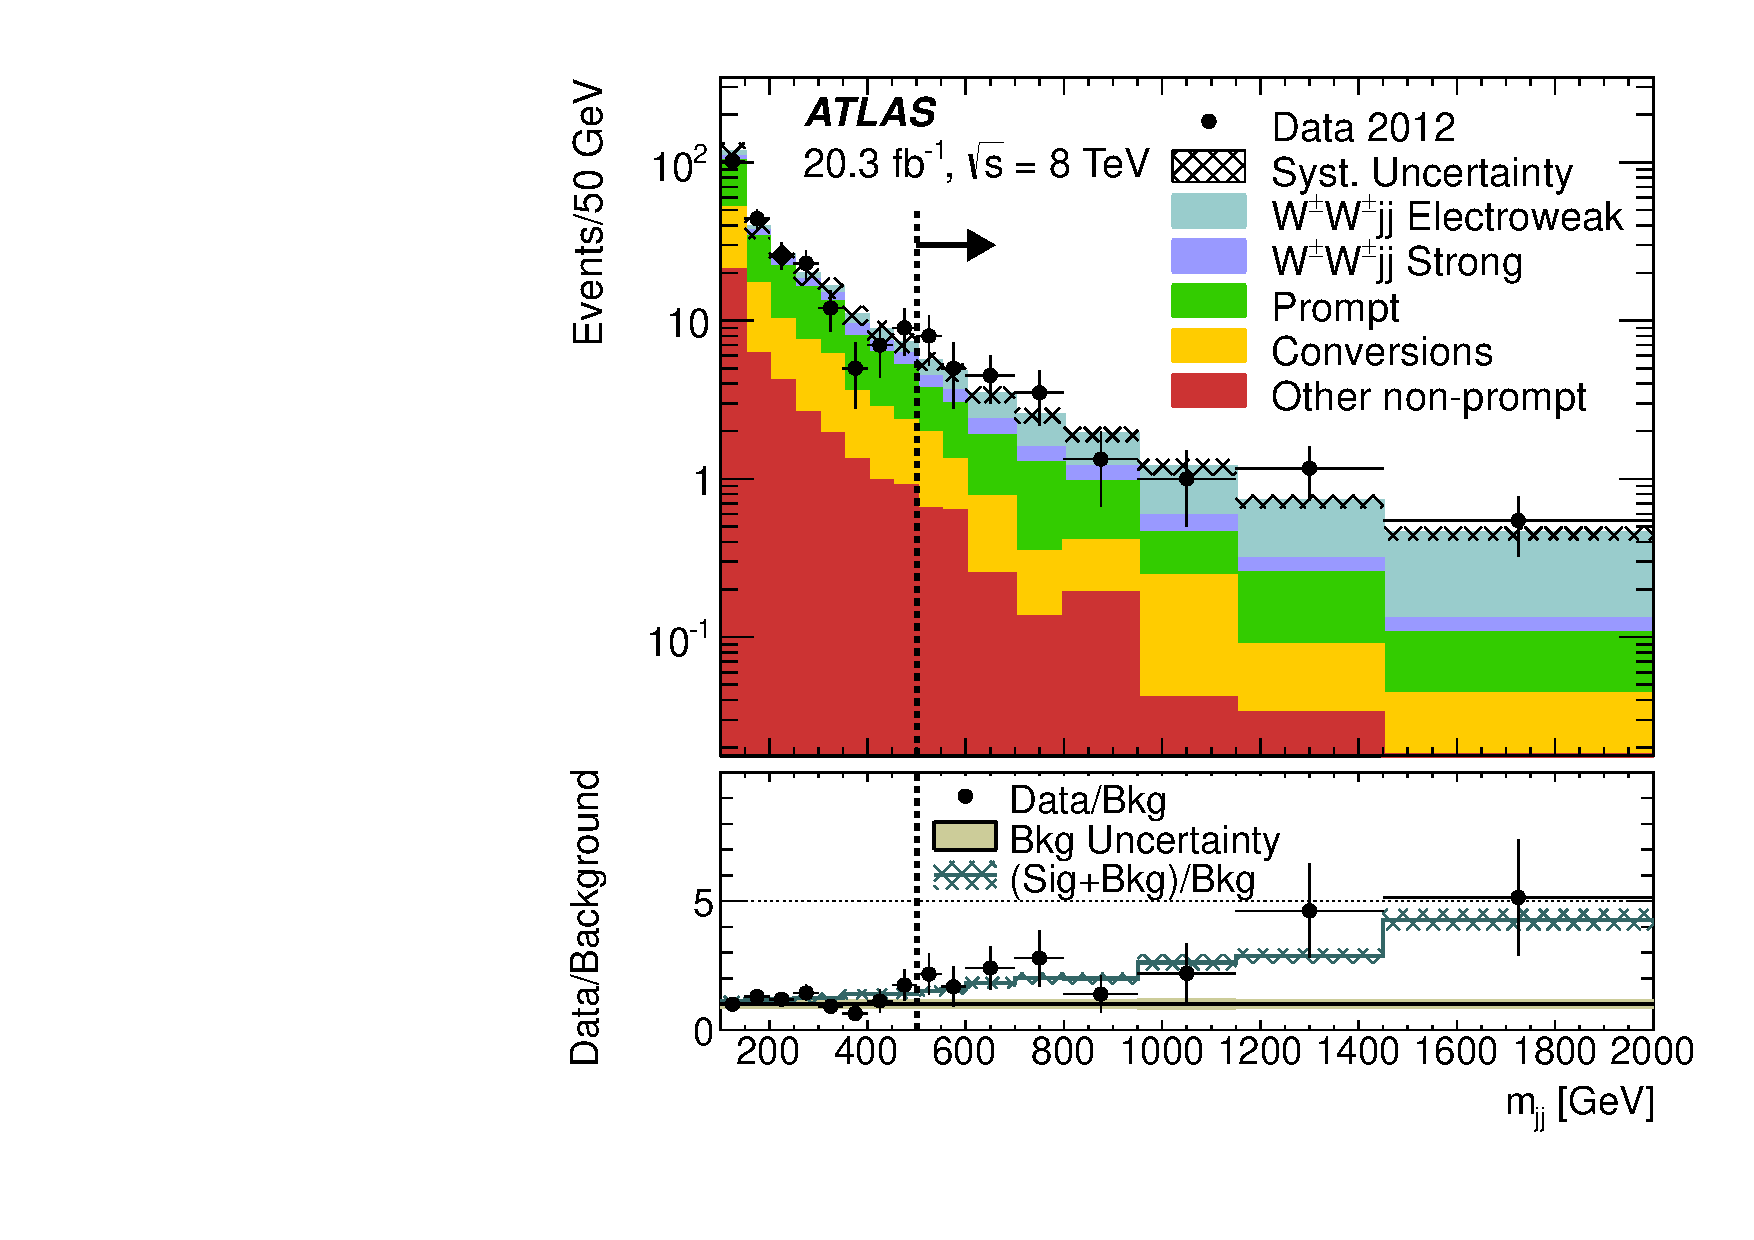
\includegraphics[width=0.45\textwidth]{figures/ss-exclboson-ww-ss-atlas8tev.pdf}
    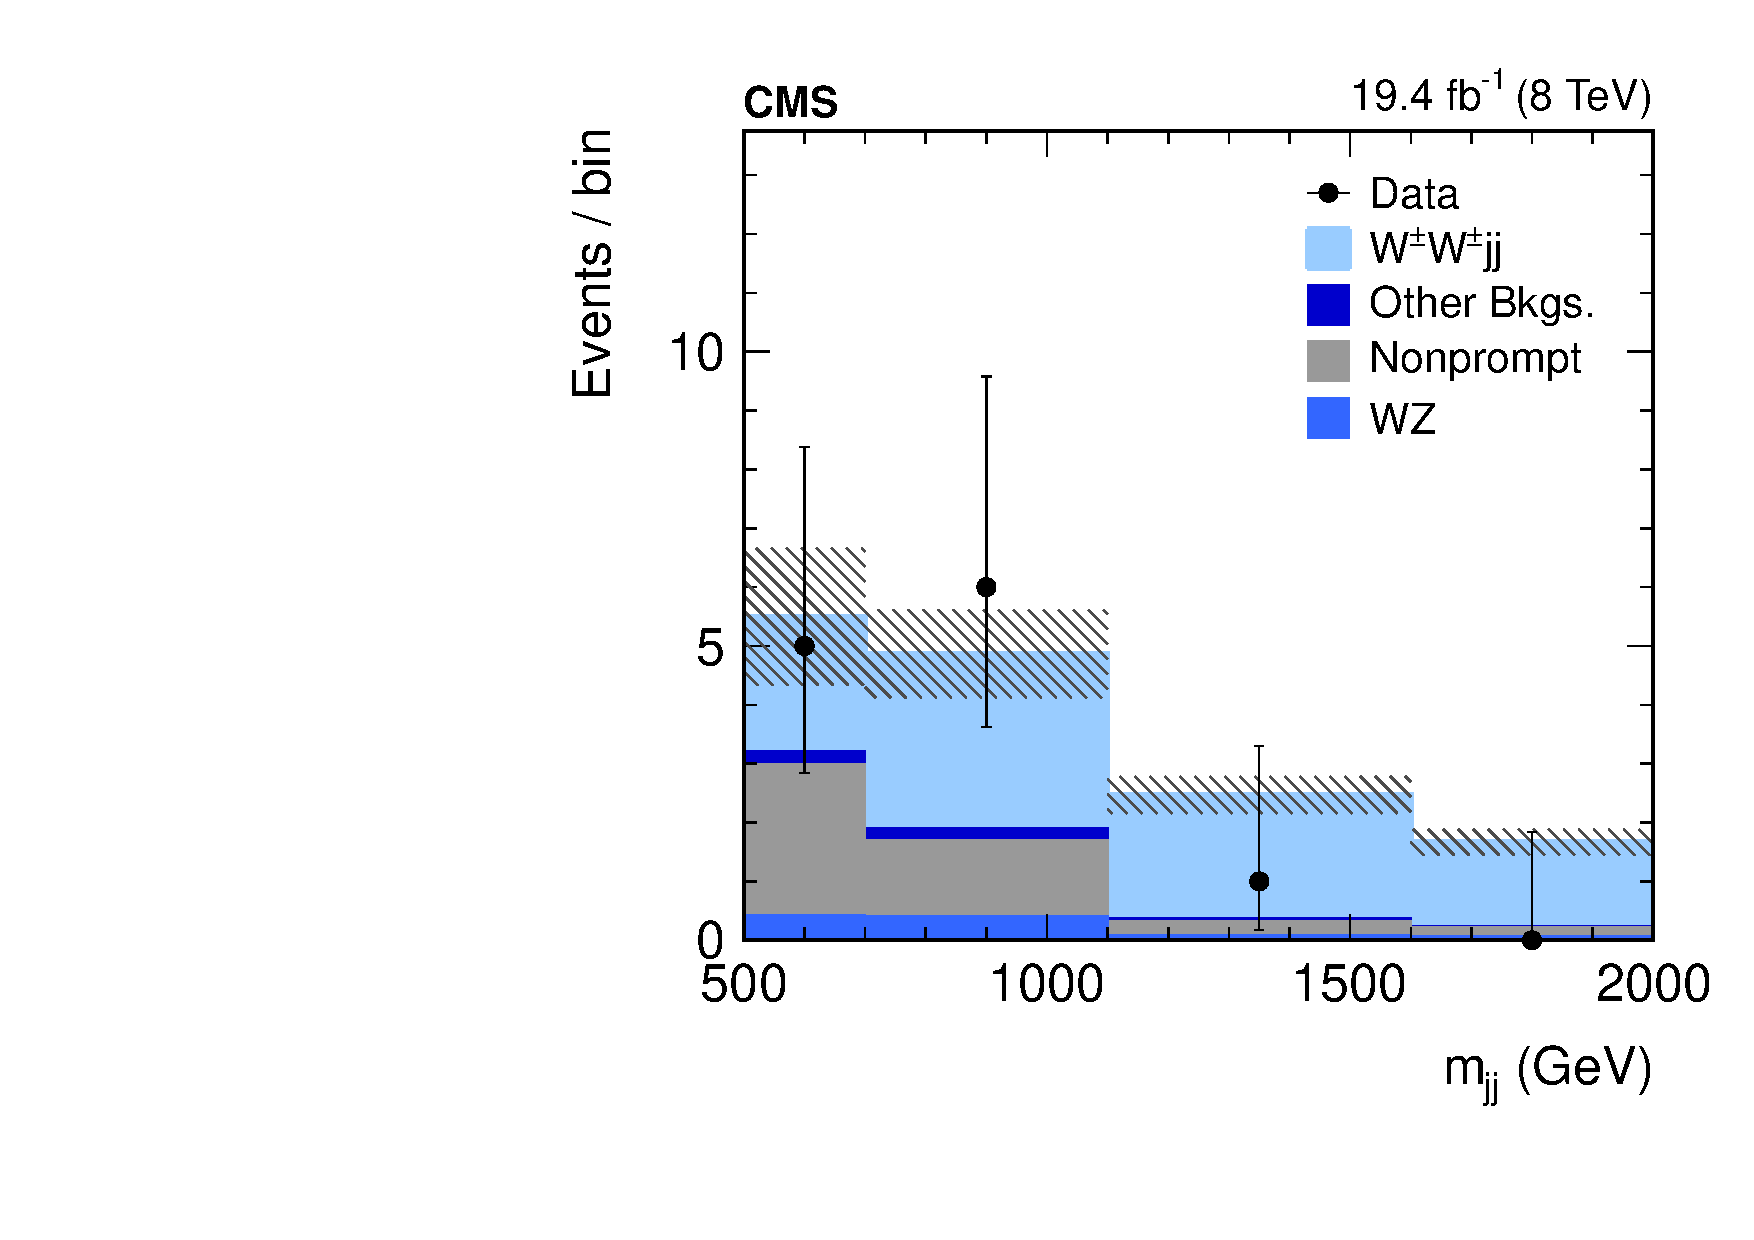
\includegraphics[width=0.45\textwidth]{figures/ss-exclboson-ww-ss-cms8tev.pdf}
    \caption{
    Left: Dijet invariant mass distribution of $W^{\pm} W^{\pm} jj$ candidates selected by ATLAS~\cite{Aad:2014zda}.  The inclusive signal region is indicated by the arrow.
    Right: Dijet invariant mass distribution of $W^{\pm} W^{\pm} jj$ candidates selected by CMS~\cite{Khachatryan:2014sta}.  }
    \label{fig:ss-exclboson-ww-ss}
\end{figure}


\section{Electroweak (precision) tests of the standard model}
\subsection{Test of tri-boson vertex}

ATLAS Wgamma Zgamma 7 \TeV~\cite{Aad:2013izg}

ATLAS WW 7 \TeV~\cite{ATLAS:2012mec}

ATLAS WW+WZ cross section 7 \TeV~\cite{Aad:2014mda}

ATLAS WZ 7 \TeV~\cite{Aad:2012twa}

ATLAS ZZ4l,ZZ2l2v 7 \TeV~\cite{Aad:2012awa}

CMS ZZ4l 8 \TeV~\cite{Khachatryan:2014dia}

CMS ZZ4l 7 \TeV~\cite{Chatrchyan:2012sga}

CMS WW2l2n 7 \TeV~\cite{Chatrchyan:2013yaa}

CMS WWlnjj 7 \TeV~\cite{Chatrchyan:2012bd}

CMS WW2l2n 8 \TeV (CMS-PAS-SMP-14-016, to be published)

CMS \Wg/\Zg 7 \TeV~\cite{Chatrchyan:2013fya}

CMS Znngamma 7 \TeV~\cite{Chatrchyan:2013nda}

CMS \Zg 8 \TeV~\cite{Khachatryan:2015kea}

CMS \ZZllvv 7+8 \TeV~\cite{Khachatryan:2015pba}

\subsection{Test of tetra-boson vertex}

ATLAS $W\gamma\gamma$ 8 \TeV~\cite{Aad:2015uqa}

ATLAS SSWW 8 \TeV~\cite{Aad:2014zda}

CMS WVgamma 8 \TeV~\cite{Chatrchyan:2014bza}

CMS WWexcl 7 \TeV~\cite{Chatrchyan:2013foa}

CMS SSWW 8 \TeV~\cite{Khachatryan:2014sta}

\subsection{Z AFB and sin thetaW}

ATLAS weak mixing angle~\cite{Aad:2015uau}

CMS weak mixing angle~\cite{Chatrchyan:2011ya}

CMS Drell--Yan AFB 7 \TeV~\cite{Chatrchyan:2012dc}

CMS Drell--Yan AFB 8 \TeV, \gz, \kz, \lz (CMS-PAS-SMP-14-004, to be published)

\subsection{W mass}

\section{Summary}


ATLAS~\cite{Aad:2008zzm}
CDF~\cite{Abulencia:2005ix}
CMS~\cite{CMSdetector}
D0~\cite{Abazov:2005pn}
LHCb~\cite{Alves:2008zz}

CDF Z asymmetry muon~\cite{Aaltonen:2014loa}
CDF Z asymmetry electron~\cite{Aaltonen:2013wcp}
CDF W mass PRD~\cite{Aaltonen:2013vwa}
CDF W mass PRL~\cite{Aaltonen:2012bp}

D0 W asymmetry electron~\cite{Abazov:2013dsa}
D0 W asymmetry muon~\cite{Abazov:2013rja}
D0 W mass PRD~\cite{D0:2013jba}
D0 W mass PRL~\cite{Abazov:2012bv}

CDF+D0 W mass combination~\cite{Aaltonen:2013iut}

Snowmass electroweak~\cite{Baak:2013fwa}

Wmass PDF~\cite{Bozzi:2011ww}

\ack
Acknowledgments go here.

\bibliographystyle{iopart-num}
\bibliography{ewkrun1_master}

\end{document}
